%Unreviewed SI

\section*{Full modeling results}
We report a full model comparison of two models of learning each combined with three different sampling strategies (see also Fig.~\ref{fig:gpfull}-\ref{fig:mtfull}). Different \emph{models of learning} (i.e., Gaussian Process regression and Mean Tracker) are combined with different \emph{sampling strategies}, in order to make predictions about where a participant will search next, given the history of previous observations. Table~\ref{tab:modelResults} contains the predictive accuracy, the number of participants best described, the log-loss, the probability of exceedance and the parameter estimates of each combination of a learning model and a sampling strategy. In total, cross-validated model comparisons for both models required approximately two days of computation time distributed on a cluster of 160 Dell C6220 nodes. 

\subsection*{Models of Learning} 
\subsubsection{Gaussian Process} 

We use Gaussian Process (GP) regression as a Bayesian model of generalization. A GP is defined as a collection of points, any subset of which is multivariate Gaussian. Let $f: \mathcal{X} \rightarrow R^n$ denote a function over input space $\mathcal{X}$ that maps to real-valued scalar outputs. This function can be modeled as a random draw from a GP:

\begin{align}
f \sim \mathcal{GP}(m,k),
\end{align}
where $m$ is a mean function specifying the expected output of the function given input $\mathbf{x}$, and $k$ is a kernel (or covariance) function specifying the covariance between outputs:

\begin{align}
m(\mathbf{x})&=\mathbb{E}[f( \mathbf{x})]\\
k(\mathbf{x}, \mathbf{x}')&=\mathbb{E}\left[(f( \mathbf{x})-m(\mathbf{x}))(f( \mathbf{x'})-m(\mathbf{x'}))\right]
\end{align} 
Here, we fix the prior mean to the median value of unscaled payoffs, $m(\mathbf{x})=25$, and use the kernel function to encode an inductive bias about the expected spatial correlations between rewards (see Radial Basis Function kernel below). 

Conditional on observed data $\mathcal{D}_t=\{\mathbf{x}_j, y_j\}_{j=1}^t$, where $y_j \sim \mathcal{N}(f(\mathbf{x}_j),\sigma_j^2)$ is drawn from the underlying function with added noise $\sigma_j^2=1$, we can calculate the posterior predictive distribution for a new input $\mathbf{x}_\ast$ as a Gaussian with mean and variance given by:
\begin{align}
\mathbb{E}[f(\mathbf{x}_\ast)|\mathcal{D}_t]&=m_t(\mathbf{x}_\ast) = \mathbf{k}_\ast^\top (\mathbf{K}+\sigma^2\mathbf{I})^{-1}\mathbf{y}_t \\
\mathbb{V}[f(\mathbf{x}_\ast)|\mathcal{D}_t]&=v_t(\mathbf{x}_\ast) = k(\mathbf{x}_\ast,\mathbf{x}_\ast)-\mathbf{k}_\star^\top(\mathbf{K}+\sigma^2\mathbf{I})^{-1}\mathbf{k}_\ast,
\end{align}
where $\mathbf{y} = [y_1,\ldots,y_t]^\top$, $\mathbf{K}$ is the $t \times t$ covariance matrix evaluated at each pair of observed inputs, and $\mathbf{k}_\ast = [k(\mathbf{x}_1,\mathbf{x}_\ast),\ldots,k(\mathbf{x}_t,\mathbf{x}_\ast)]$ is the covariance between each observed input and the new input $\mathbf{x}_\ast$.

\subsubsection{Radial Basis Function kernel} 
We use the Radial Basis Function (RBF) kernel as a component of the $\mathcal{GP}$ algorithm of generalization. The RBF kernel specifies the correlation between inputs $\mathbf{x}$ and $\mathbf{x}'$ as

\begin{align}
k(\mathbf{x}, \mathbf{x}')=\exp\left(-\frac{||\mathbf{x}-\mathbf{x}'||^2}{\lambda}\right).
\end{align}

This kernel defines a universal function learning engine based on the principles of Bayesian regression and can theoretically model any stationary function. Note that sometimes the RBF kernel is specified as $k(\mathbf{x}, \mathbf{x}')=\exp\left(-\frac{||\mathbf{x}-\mathbf{x}'||^2}{2l^2}\right)$ whereas we use $\lambda = 2l^2$ as a more psychologically interpretable formulation. Intuitively, the RBF kernel models the correlation between points as an exponentially decreasing function of their distance. Here, $\lambda$ modifies the rate of correlation decay, with larger $\lambda$-values corresponding to slower decays, stronger spatial correlations, and smoother functions. As $\lambda \to \infty$, the RBF kernel assumes functions approaching linearity, whereas as $\lambda \to 0$, there ceases to be any spatial correlation, with the implication that learning happens independently for each discrete input without generalization (similar to the assumption of the Mean Tracker model described below). We treat $\lambda$ as a free parameter, and use cross-validated estimates to make inferences about the extent to which participants generalize.

\subsubsection*{Mean Tracker} 

The Mean Tracker model is implemented as a Bayesian updating model, which assumes the average reward associated with each option is constant over time (i.e., no temporal dynamics), as is the case in our experiment. In contrast to the GP regression model (which also assumes constant means over time), the Mean Tracker learns the rewards of each option independently, by computing an independent posterior distribution for the mean $\mu_j$ for each option $j$. We implemented a version that assumes rewards are normally distributed (as in the GP model), with a known variance but unknown mean, where the prior distribution of the mean is a normal distribution. This implies that the posterior distribution for each mean is also a normal distribution: 
\begin{align}
p(\mu_{j,t}|\mathcal{D}_{t-1}) &= \mathcal{N}(m_{j,t},v_{j,t})
\end{align}
For a given option $j$, the posterior mean $m_{j,t}$ and variance $v_{j,t}$ are only updated when it has been selected at trial $t$:

\begin{align}
m_{j,t} &= m_{j,t-1} + \delta_{j,t}G_{j,t}\left[y_t-m_{j,t-1}\right]\\
v_{j,t} &= \left[1 - \delta_{j,t}G_{j,t}\right]v_{j,t-1} 
\end{align}
where $\delta_{j,t}=1$ if option $j$ is chosen on trial $t$, and $0$ otherwise. Additionally, $y_t$ is the observed reward at trial $t$, and $G_{j,t}$ is defined as:

\begin{align}
G_{j,t} &= \frac{v_{j,t-1}}{v_{j,t-1}+ \theta_\epsilon^2}
\end{align}
where $\theta_\epsilon^2$ is the error variance, which is estimated as a free parameter. Intuitively, the estimated mean of the chosen option $m_{j,t}$ is updated based on the difference between the observed value $y_t$ and the prior expected mean $m_{j,t-1}$, multiplied by $G_{j,t}$. At the same time, the estimated variance $v_{j,t}$ is reduced by a factor of $1 - G_{j,t}$, which is in the range $[0,1]$. The error variance ($\theta_\epsilon^2$) can be interpreted as an inverse sensitivity, where smaller values result in more substantial updates to the mean $m_{j,t}$, and larger reductions of uncertainty $v_{j,t}$. We set the prior mean to the median value of unscaled payoffs $m_{j,0}=25$ and the prior standard deviation to $\sqrt{v_{j,0}}=250$.

\subsection*{Sampling strategies} \hspace*{\fill} \\ 
Given the normally distributed posteriors of the expected rewards, which have mean $\mu(\mathbf{x})$ and uncertainty (formalized here as standard deviation) $\sigma(\mathbf{x})$, for each search option $\mathbf{x}$ (for the Mean Tracker, we let $\mu(\mathbf{x}) = m_{j,t}$ and $\sigma(\mathbf{x}) = \sqrt{v_{j,t}}$, where $j$ is the index of the option characterized by $\mathbf{x}$), we assess different sampling strategies that (combined with a softmax choice rule, Eq.~\ref{eq:softmax}) make probabilistic predictions about where participants would search next. 

\subsubsection{Upper Confidence Bound sampling} 
Given the posterior predictive mean $\mu(\mathbf{x})$ and its attached standard deviation $\sigma(\mathbf{x}) = \sqrt{\sigma^2(\mathbf{x})}$, we calculate the upper confidence bound using a weighted sum
\begin{align}
\text{UCB}(\mathbf{x})&=\mu(\mathbf{x})+\beta \sigma(\mathbf{x}),
\end{align}
where the exploration factor $\beta$ determines how much reduction of uncertainty is valued (relative to exploiting known high-value options). We estimate $\beta$ as a free parameter indicating participants' tendency towards directed exploration.

\subsubsection{Mean Greedy Exploitation} 
A special case of the Upper Confidence Bound sampling strategy (with $\beta=0$) is a greedy exploitation component that only evaluates points based on their expected rewards
\begin{align}
\text{M}(\mathbf{x})&=\mu(\mathbf{x}), 
\end{align}
This sampling strategy only samples options with high expected rewards, i.e. greedily exploits the environment.

\subsubsection{Variance Greedy Exploration} 
Another special case of the Upper Confidence Bound sampling strategy (with $\beta \to \infty$) is a greedy exploration component which only samples points based on their predictive standard deviation
\begin{align}
\text{V}(\mathbf{x})=\sigma(\mathbf{x}).
\end{align}
This sampling strategy only cares about reducing uncertainty without attempting to generate high rewards.

\section*{Model comparison}
We use maximum likelihood estimation (MLE) for parameter estimation, and cross-validation to measure out-of-sample predictive accuracy. A softmax choice rule transforms each model's predictions into a probability distribution over options:
\begin{align}
p(\mathbf{x}) &= \frac{\exp(q(\mathbf{x})/\tau)}{\sum_{j=1}^{N}\exp(q(\mathbf{x}_j)/\tau)},
\label{eq:softmax}
\end{align}
where $q(\mathbf{x})$ is the predicted value of each option $\mathbf{x}$ for a given model (e.g., $q(\mathbf{x}) = \text{UCB}(\mathbf{x})$ for the UCB model), and $\tau$ is the temperature parameter. Lower values of $\tau$ indicate more concentrated probability distributions, corresponding to more precise predictions and therefore less random sampling. All models include $\tau$ as a free parameter. Additionally, we estimate $\lambda$ (generalization parameter) for the Gaussian Process regression model and $\theta^2_\epsilon$ (error variance) for the Mean Tracker model. Finally, we estimate $\beta$ (exploration bonus) for the Upper Confidence Bound sampling strategy.

\subsubsection*{Cross validation} 
We fit all combinations of models and sampling strategies---per participant---using cross-validated MLE implemented via a Differential Evolution algorithm for optimization. Parameter estimates are constrained to positive values in the range $[\exp(-5),\exp(5)]$. We use leave-one-round-out cross-validation to iteratively form a training set by leaving out a single round, computing a MLE on the training set, and then generating out-of-sample predictions on the remaining round. This is repeated for all combinations of training set and test set. This cross-validation procedure yields one set of parameter estimates per round, per participant, and out-of-sample predictions for 200 choices per participant overall (rounds 2-9 $\times$ 25 choices). 

\subsubsection*{Predictive accuracy}  
Prediction error (computed as log loss) is summed up over all rounds (apart from the tutorial and the bonus rounds), and is reported as \emph{predictive accuracy}, using a pseudo-$R^2$ measure that compares the total log loss prediction error for each model to that of a random model: 
\begin{align}
R^2=1-\frac{\log\mathcal{L}(\mathcal{M}_k)}{\log\mathcal{L}(\mathcal{M}_{\text{rand}})},
\end{align}
where $\log\mathcal{L}(\mathcal{M}_{\text{rand}})$ is the log loss of a random model (i.e., picking options with equal probability) and $\log\mathcal{L}(\mathcal{M}_k)$ is the log loss of model $k$'s out-of-sample prediction error. Intuitively, $R^2=0$ corresponds to prediction accuracy equivalent to chance, while $R^2=1$ corresponds to theoretical perfect predictive accuracy, since $\log\mathcal{L}(\mathcal{M}_k)/\log\mathcal{L}(\mathcal{M}_{\text{rand}}) \to 0$ when $\log\mathcal{L}(\mathcal{M}_k) \ll \log\mathcal{L}(\mathcal{M}_{\text{rand}})$. 





\subsection*{Parameter estimates}  

All parameter estimates were included in the statistical analyses, although we exclude outliers larger than 5 in Figures 1e, \ref{fig:paramRecover}, \ref{fig:gpfull}, \ref{fig:mtfull}, and in Table~\ref{tab:modelResults}. For GP-UCB estimates, 1.1\% of $\lambda$-estimates, for 3.4\% of $\beta$-estimates, and 2.7\% of $\tau$-estimates were removed this way. The presence of these outliers motivated us to use non-parametric tests (without removing outliers) to compare the different parameters across age groups, in order to achieve more robustness. However, the significance of our test results does not change even if we use parametric $t$-tests, but remove outliers before performing these tests. After removing values higher than 5, we still find that adults show higher $\lambda$-estimates than older children ($t(103)=3.88$, $p<.001$, $d=0.76$, 95\% CI=$[0.36,1.16]$, $BF>100$), who do not differ in their $\lambda$-estimates from younger children ($t(108)=1.00$, $p=.32$, $d=0.19$, 95\% CI=$[-0.19,0.57]$, $BF=0.3$). Moreover, the $\beta$-estimates are higher for older children than for adults ($t(103)=4.41$, $p<.001$, $d=0.87$, 95\% CI=$[0.46,1.28]$, $BF>100$), but do not differ between the two groups of children $t(108)=1.41$, $p=.160$, $d=0.27$, 95\% CI=$[-0.11,0.66]$, $BF=0.5$). Crucially, the random exploration parameters $\tau$ do neither differ between older children and adults ($t(103)=.55$, $p=.58$, $d=0.11$, 95\% CI=$[-0.28,0.50]$, $BF=0.2$), nor do they differ between the two groups of children ($t(108)=1.74$, $p=.08$, $d=0.33$, 95\% CI=$[-0.72,0.05]$, $BF=0.8$).

Our criterion for outlier removal is less strict than other criteria, such as removing values higher than 1.5$\times$IQR. In our data, this would remove 1.8\% of $\lambda$-estimates, 5.1\% of $\beta$-estimates, and 11.2\% of $\tau$-estimates. For completeness, we also reanalyzed the data after performing Tukey's procedure of outlier removal, where we find the same results. Adults still show a higher $\lambda$-estimates than older children ($t(102)=3.87$, $p<.001$, $d=0.76$, 95\% CI=$[0.36,1.17]$, $BF>100$), who do not differ from younger children ($t(108)=1.04$, $p=.30$, $d=0.20$, 95\% CI=$[-0.18, 0.58]$, $BF=0.3$). The $\beta$-estimates are again higher for older children than for adults ($t(100)=4.69$, $p<.001$, $d=0.93$, 95\% CI=$[0.51, 1.34]$, $BF>100$), and do not differ between the two groups of children ($t(103)=1.06$, $p=.29$, $d=0.21$, 95\% CI=$[-0.18, 0.60]$, $BF=0.3$). Finally, estimates for $\tau$-parameter do not differ between adults and older children ($t(103)=1.36$, $p=.18$, $d=0.26$, 95\% CI=$[-0.12, 0.66]$, $BF=0.5$), nor between the two groups of children ($t(108)=0.96$, $p=.34$, $d=0.18$, 95\% CI=$[-0.38, 0.38]$, $BF=0.3$). Taken together, our results hold no matter which method of outlier removal is applied.

\section*{Full model comparison results}
\begin{figure}[ht!]
\centering
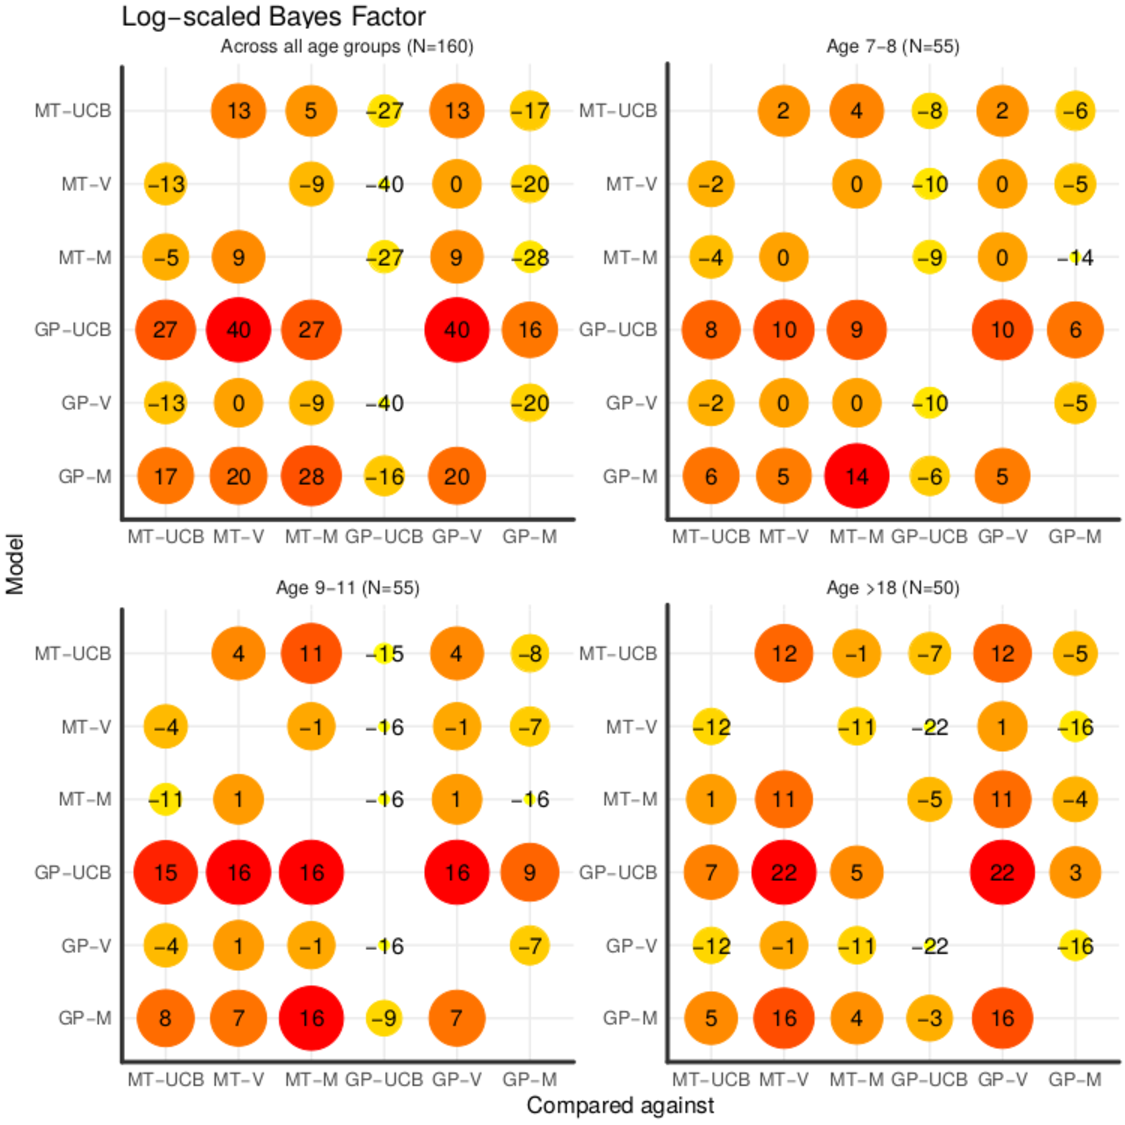
\includegraphics[width=0.8\linewidth]{bayesfactor.pdf}
\caption{Log-scaled Bayes factor for every pair-wise model comparison, between a model on the y-axis compared against a model on the x-axis. Numbers indicate $\log_{10}$ of the Bayes Factor, with a value of 1 indicating that the alternative hypothesis is around 10-times more likely than the null hypothesis, whereas a value of -1 means that the null hypothesis is around 10-times more likely than the alternative hypothesis. Larger Bayes Factors are accompanied by larger circles and darker shades of red. Comparisons show both learning models---the Gaussian Process (GP) and the Mean Tracker (MT)---combined with every sampling strategy, Upper Confidence Bound sampling (UCB), Variance-greedy sampling (V), and Mean-greedy sampling (M).} 
\label{fig:bayesfactor}
\vspace{-1mm}
\end{figure}

Figure~\ref{fig:bayesfactor} shows the log-scaled Bayes Factor of every combination of each learning model with each sampling strategy, compared in terms of predictive accuracy to every other combination, and separated by the different age groups. Results are based on one-sided Bayesian $t$-tests. We find that the GP-UCB model wins against every other combination, resulting in large Bayes factors overall, but also for every individual age group. 


\begin{figure}[ht!]
\centering
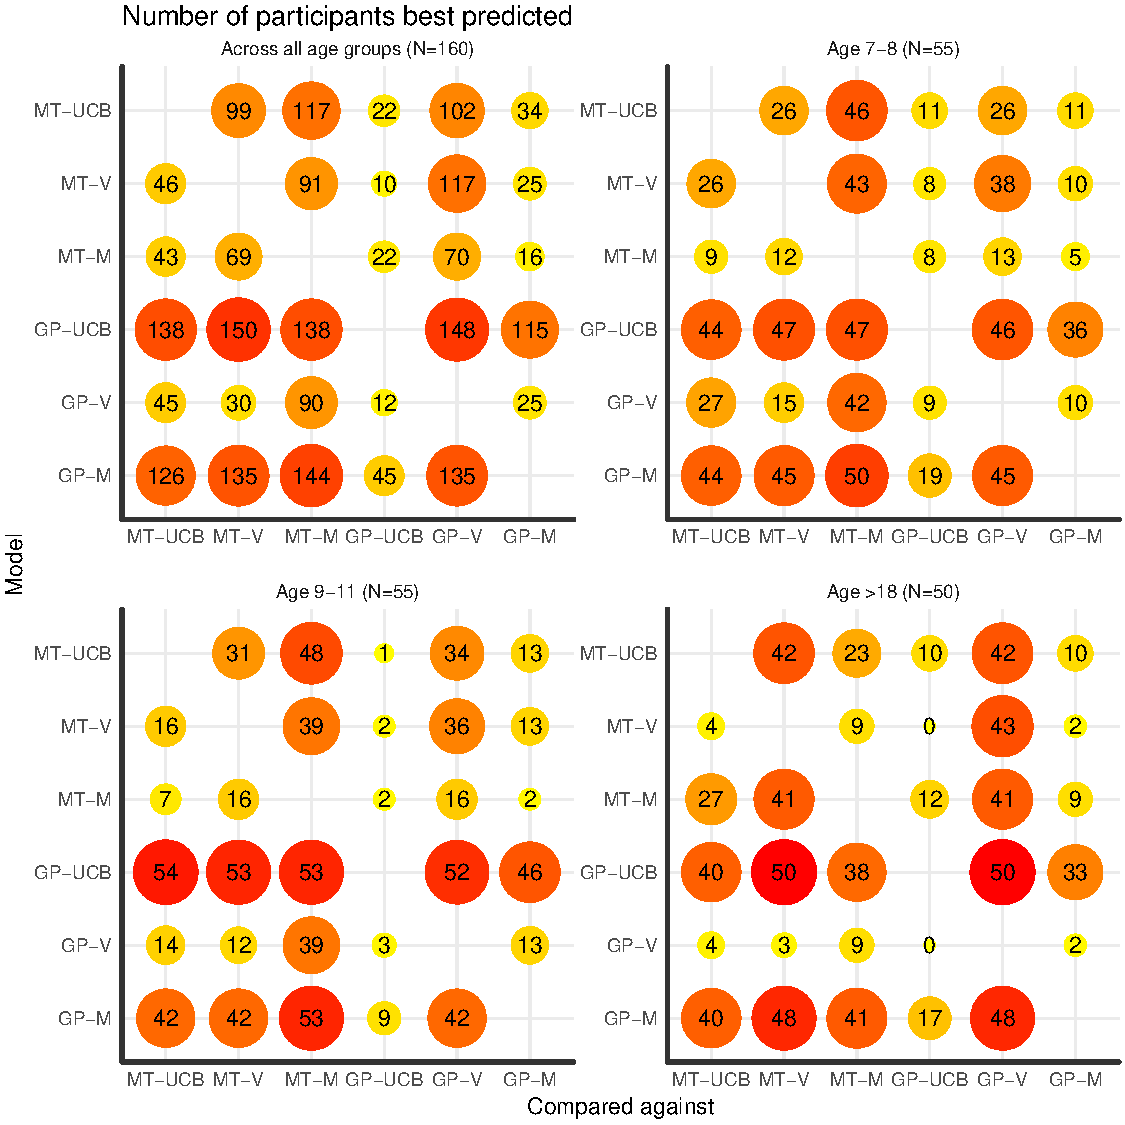
\includegraphics[width=0.8\linewidth]{bestdescribed.pdf}
\caption{Number of participants best predicted for every pair-wise model comparison, comparing a model on the y-axis with a model on the x-axis. Numbers show absolute counts and can only be interpreted in relation to the overall number of participants per group (shown in brackets at the top of each panel). A larger proportion of participants best predicted are accompanied by larger circles and darker shades of red. Comparisons show both models---the Gaussian Process (GP) and the Mean Tracker (MT)--- combined with every sampling strategy, Upper Confidence Bound sampling (UCB), Variance-greedy sampling (V), and Mean-greedy sampling (M).} 
\label{fig:bestpredict}
\vspace{-1mm}
\end{figure}

In addition to these Bayes factors for comparisons between individual models, we also compare the cross-validated log-loss at the group level using (predictive) Bayesian model selection, estimating each model's protected probability of exceedance, which is the likelihood that the proportion of participants generated using a given combination exceeds the proportion of participants generated using all other combinations, while controlling for the chance rate. This analysis revealed that the overall hypothesis of all models performing equally well was rejected by a Bayesian omnibus test at $p<.001$. Moreover, the protected probability of exceedance was virtually 1 for the GP-UCB model, where 1 is the upper theoretical limit. This result is also obtained if breaking down the analysis by the different age groups, again always leading to a protected probability of exceedance of 1 for the GP-UCB model.

Finally, we report how many participants are best predicted by each combination of a model and a sampling strategy. The results of this comparison are shown in Figure~\ref{fig:bestpredict} (see also Table~\ref{tab:modelResults}). As before, the GP-UCB model is the best overall model and also predicts most participants best for every age group. Overall, the GP-UCB model predicted 106 out of 160 participants best. In the different age categories, the GP-UCB model best predicted 32 out of 55 younger children, 44 out of 55 older children, and 30 out of 50 adult participants. Therefore, the GP-UCB model was by far the best model in our comparison.




\section*{Model recovery}

We present model recovery results that assess whether or not our predictive model comparison procedure allows us to correctly identify the true underlying model. To assess this, we generated data based on each individual participant's mean parameter estimates (excluding outliers larger than 5 as before). More specifically, for each participant and round, we use the cross-validated parameter estimates to specify a given model, and then generate new data in the attempt to mimic participant data. We generate data using the Mean Tracker and the GP regression model. In all cases, we use the UCB sampling strategy in conjunction with the specified learning model. We then utilize the same cross-validation method as before in order to determine if we can successfully identify which model has generated the underlying data. Figure~\ref{fig:recovercompare} shows the cross-validated predictive performance for the simulated data. 

\subsection*{Recovery Results} \hspace*{\fill} \\
\begin{figure}[ht!]
\centering
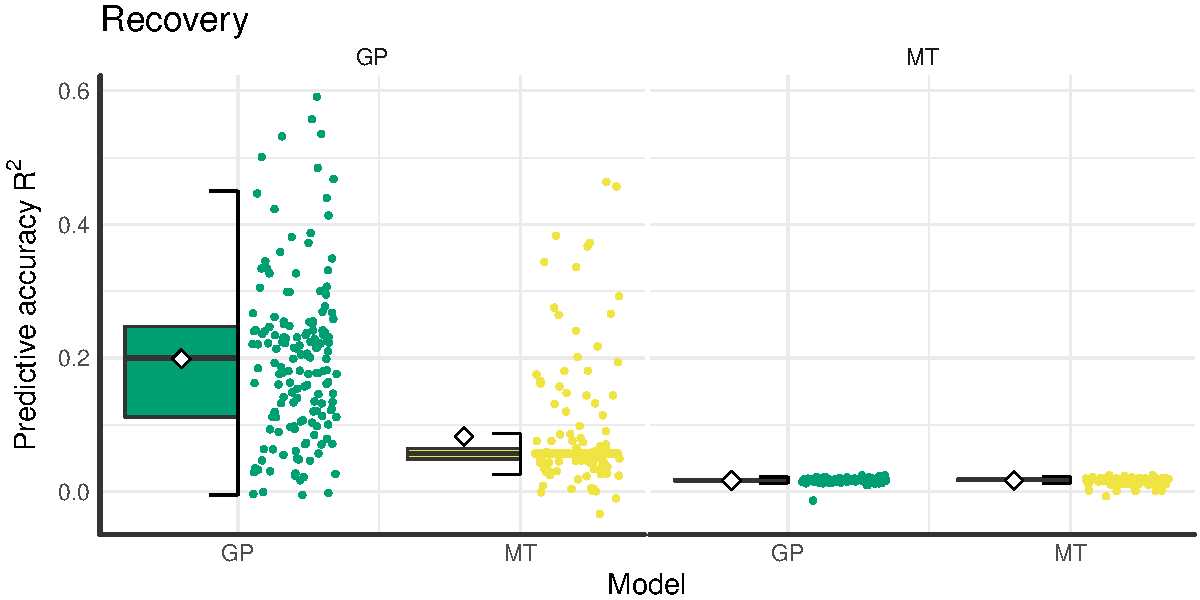
\includegraphics[width=0.8\linewidth]{recoverycompare.pdf}
\caption{Tukey box plots of model recovery results including individual data points (points) and overall means (diamonds). \textbf{Left:} Model performance based on data generated by the GP-UCB model specified with participant parameter estimates. The matching GP-UCB model makes better predictions than a mismatched MT-UCB model. \textbf{Right:} Model performance based on data generated by the MT-UCB model specified with participant parameter estimates. Both GP and MT models predict this data poorly, and perform similar to a random model.} 
\label{fig:recovercompare}
\vspace{-1mm}
\end{figure}

Our predictive model comparison procedure shows that the Gaussian Process model is a better predictor for data generated from the same underlying model, whereas the Mean Tracker model is only marginally (if at all) better at predicting data generated from the same underlying model. This suggests that our main model comparison results are robust to Type II errors, and provides evidence that the better predictive accuracy of the GP model on participant data is unlikely due to differences in model mimicry.

When the Mean Tracker model generates data using participant parameter estimates, the same Mean Tracker model performs better than the GP model ($t(159)=1.42$, $p=.16$, $d=0.11$, 95\% CI=$[-0.12, 0.33]$, $BF=4.1$) and predicts 86 out of 160 simulated participants best. Notice, however, that both models perform poorly in this case, with both models achieving an average pseudo-r-squared of around $R^2=-0.04$. This also shows that the Mean Tracker is not a good generative model of human-like behavior in our task.

When the Gaussian Process regression model has generated the underlying data, the same model performs significantly better than the Mean Tracker model ($t(159)=18.6$, $p<.001$, $d=1.47$, 95\% CI=$[1.22, 1.72]$, $BF>100$) and predicts 153 of the 160 simulated participants best. In general, both models perform better when the GP has generated the data with the GP achieving a predictive accuracy of $R^2=.20$ and the MT of achieving $R^2=.12$. This makes our finding of the Gaussian Process regression model as the best predictive model even stronger as --technically-- the Mean Tracker model can mimic parts of its behavior. Moreover, the resulting values of predictive accuracy are similar to the ones we found using participant data. This indicates that our empirical values of predictive accuracy were as good as possible under the assumption that a GP model generated the data.



\section*{Parameter Recovery} 
\begin{figure}[ht!]
\centering
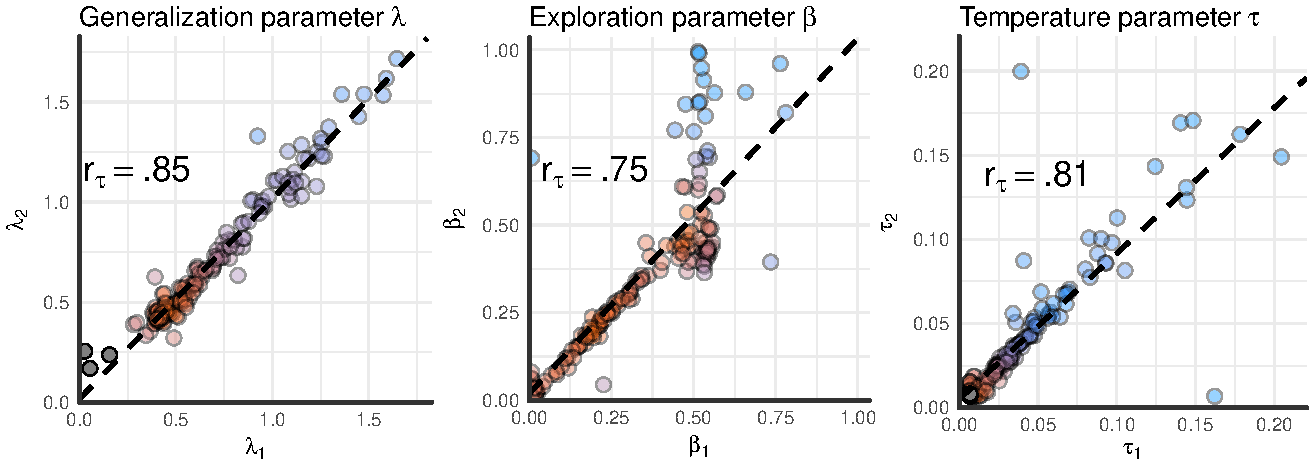
\includegraphics[width=0.8\linewidth]{recovery.pdf}
\caption{Parameter recovery results. The generating parameter estimate is on the x-axis and the recovered parameter estimate is on the y-axis. The generating parameter estimates are from the cross-validated participant parameter estimates, which were used to simulate data (see Model recovery). Recovered parameter estimates are the result of the cross-validated model comparison (see Model comparison) on the simulated data. While the cross-validation procedure yielded $8$-estimates per participant, one for each round, we show the mean estimate per (simulated) participant. The dashed line shows a linear regression on the data, while Kendall's rank correlation $r_\tau$ is shown in the plot. For readability, colors represent the bivariate kernel density estimate, with red indicating higher density.} 
\label{fig:paramRecover}
\vspace{-1mm}
\end{figure}

Another important question is whether the reported parameter estimates of the GP-UCB model are reliable and recoverable. We address this question by assessing the recoverability of the three underlying parameters, the length-scale $\lambda$, the directed exploration factor $\beta$, and the random exploration (temperature) parameter $\tau$ of the softmax choice rule. We use the results from the model recovery simulation described above, and correlate the empirically estimated parameters used to generate data (i.e., the estimates based on participants' data), with the parameter estimates of the recovering model (i.e., the MLE from the cross-validation procedure on the simulated data). We assess whether the recovered parameter estimates are similar to the parameters that were used to generate the underlying data. We present parameter recovery results for the Gaussian Process regression model using the UCB sampling strategy. We report the results in Figure~\ref{fig:paramRecover}, with the generating parameter estimate on the x-axis and the recovered parameter estimate on the y-axis.

The correlation between the generating and the recovered length-scale $\lambda$ is $r_\tau=.85$, 95\% CI=$[0.81,0.90]$, $p<.001$, the correlation between the generating and the recovered exploration factor $\beta$ is $r_\tau=0.75$, 95\% CI=$[0.68,0.82]$, $p<.001$, and the correlation between the generating and the recovered softmax temperature parameter $\tau$ is $r_\tau=0.81$, 95\% CI=$[0.76,0.87]$, $p<.001$. 

These results show that the correlation between the generating and the recovered parameters is very high for all parameters. Thus, we have strong evidence to support the claim that the reported parameter estimates of the GP-UCB model are recoverable, reliable, and therefore interpretable. Importantly, we find that estimates for $\beta$ (exploration bonus) and $\tau$ (softmax temperature) are indeed recoverable, providing evidence for the existence of a \emph{directed} exploration bonus, as a separate phenomena from \emph{random} exploration in our behavioral data.

Next, we analyze whether or not the same differences between the parameter estimates that we found for the experimental data can also be found for the simulated data. Thus, we compare the recovered parameter estimates from the data generated by the estimated parameters for the different age groups. This comparison shows that the recovered data exhibits the same characteristics as the empirical data. The recovered $\lambda$-estimates for simulated data from adults was again larger than the recovered lambda estimates for older children ($U=2021$, $r_\tau=0.33$, 95\% CI=$[0.20,0.48]$, $p<.001$, $BF>100$), whereas there was no difference between the recovered parameters for the two simulated groups of children ($U=1800$, $p=.08$, $r_\tau=0.14$, 95\% CI=$[-.02,0.29]$, $BF=1$). As in the empirical data, the recovered estimates also showed a difference between age groups in their directed exploration behavior such that the recovered $\beta$ was higher for simulated older children than for simulated adults ($U=730$, $p<.001$, $r_\tau=0.33$, 95\% CI=$[0.20,0.47]$, $BF>100$), whereas there was no difference between the two simulated groups of children ($U = 1730$, $p=.19$, $r_\tau= 0.10$, 95\% CI=$[-0.05,0.26]$, $BF=0.6$). There was no difference between the different recovered $\tau$-parameters (max-$BF=0.5$). Thus, our model can also reproduce similar group differences between generalization and directed exploration as found in the empirical data.

\subsection{Counter-factual parameter recovery}
Another explanation of the finding that children differ from adult participants in their directed exploration parameter $\beta$ but not in their random exploration parameter $\tau$ could be that the softmax temperature parameter $\tau$ can sometimes track more of the random behavioral difference between participants than the directed exploration parameter $\beta$. If the random exploration parameter $\tau$ indeed tends to absorb more of the random variance in the data than the directed exploration parameter $\beta$, then perhaps one is always more likely to find differences in $\beta$ rather than differences in $\tau$. To assess this claim, we simulate data using our GP-UCB model as before but swap participants' parameter estimates of $\beta$ with their estimates of $\tau$ and vice versa. Ideally, this simulation can reveal whether it is possible for our method to find differences in $\tau$ but not $\beta$ in a counter-factual parameter recovery where the age groups differ in their random but not their directed exploration behavior. Thus, we generate data from the swapped GP-UCB model and then use our model fitting procedure to assess the GP-UCB model's parameters from this generated data. The results of this simulation reveal that simulated adults do not differ from simulated older children in their estimated directed exploration parameters $\beta$ ($U=1170$, $r_\tau=0.11$, 95\% CI=$[-0.05,0.27]$, $p=.19$, $BF=0.7$). Furthermore, the two simulated children groups also do not differ in terms of their directed exploration parameter $\beta$ ($U=1696$,$r_\tau=0.09$, 95\% CI=$[-0.07,0.25]$, $p=.27$, $BF=0.4$). However, the random exploration parameter $\tau$ is estimated to be somewhat higher for simulated older children than for simulated adults ($U=1771$, $r_\tau=0.21$, 95\% CI=$[0.06,0.36]$, $p=.01$, $BF=2.5$) and shows no difference between the two simulated children groups ($U=1631$, $p=.48$, $r_\tau=0.06$, 95\% CI=$[-0.10,0.21]$, $BF=0.4$). This means that the GP-UCB model can pick up on differences in random exploration as well and therefore that our findings are unlikely due to a false positive.

\section*{Comparison to optimal parameter estimates}
\begin{figure}[ht!]
\centering
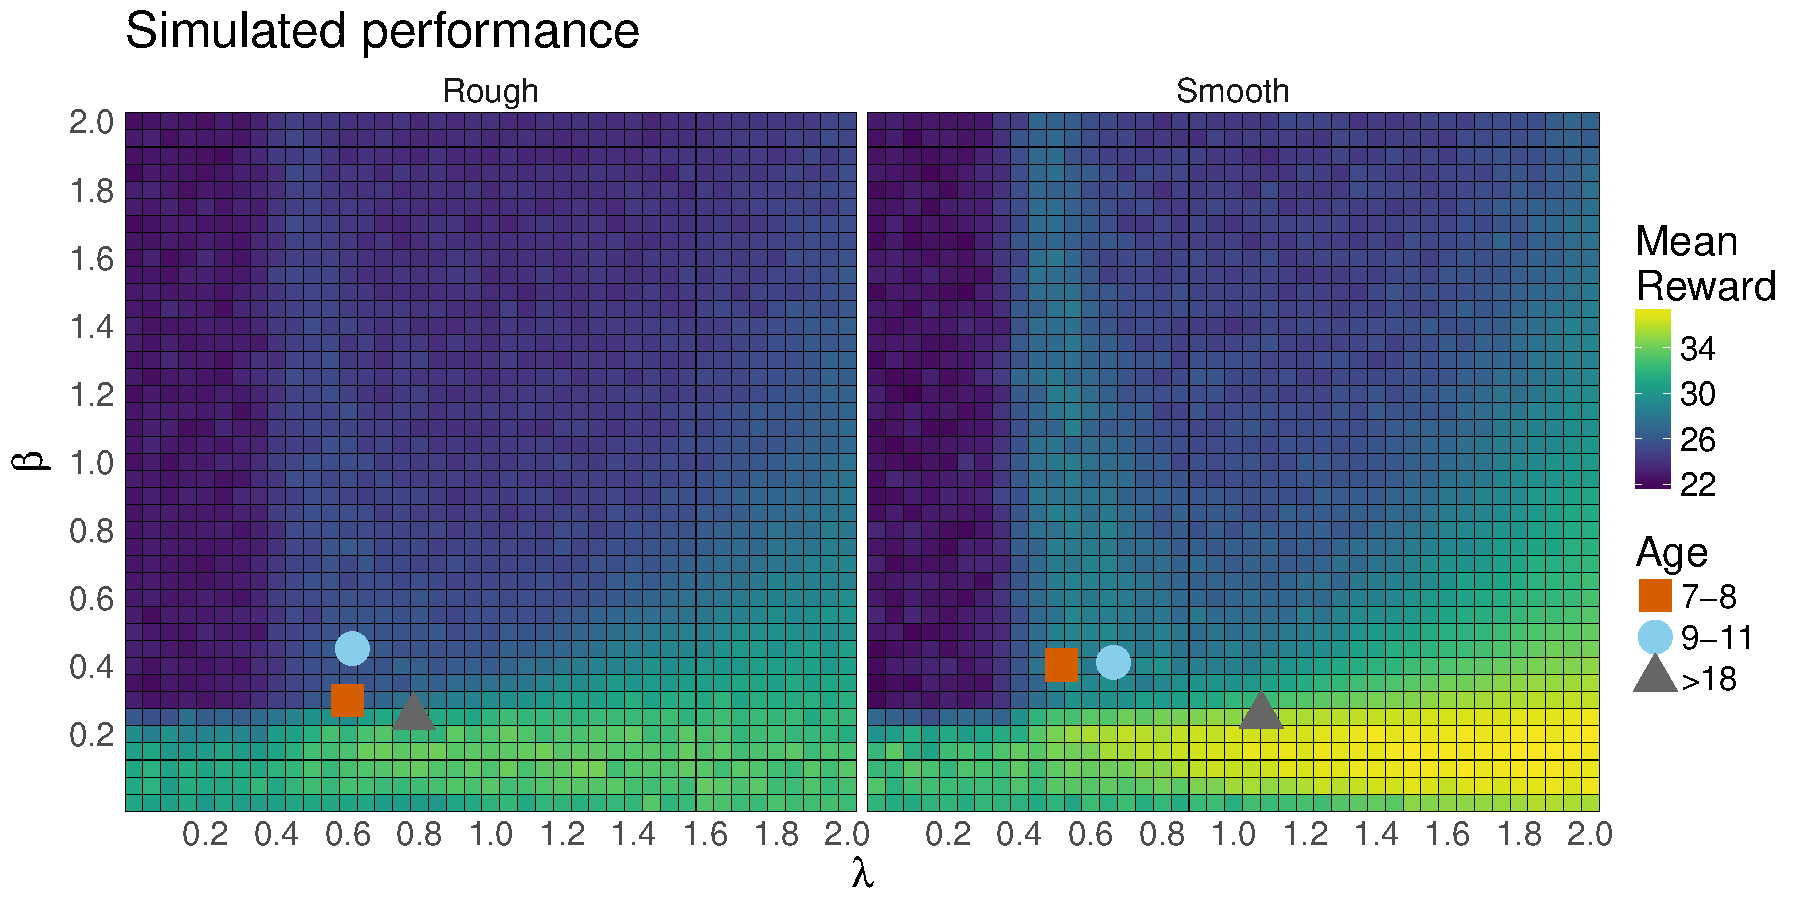
\includegraphics[width=0.9\linewidth]{simperf.pdf}
\caption{Simulated performance for different parameter values of $\lambda$ (generalization) and $\beta$ (directed exploration bonus) in the rough (left) and smooth (right) environment. Each tile shows the mean performance over 100 replications on each environment type. The mean participant parameter estimates (separated by age group) are overlaid.} 
\label{fig:optimalparams}
\vspace{-1mm}
\end{figure}

We compare participants' parameter estimates to optimally-performing estimates of the GP-UCB model (Fig.~\ref{fig:optimalparams}). For this, we simulate the GP-UCB model on both the smooth and the rough environments for the same number of trials as participants experienced, and track performance for each run. Since there were no meaningful differences for the random exploration parameter $\tau$, we set $\tau=0.03$ (i.e., the median over all participants) for all simulations. We vary the parameter values of the directed exploration bonus $\beta$ and the generalization parameter $\lambda$ to all permutations of values stemming from $[0.05,0.1,\cdots, 2]$, leading to 1,600 differently parameterized models in total. We then run each model for 100 replications on both the smooth and the rough environments individually, always calculating mean performance over all runs. Figure S5 shows the performance of different $\lambda$-$\beta$-combinations with participants' parameter estimates overlaid.


We extract the best parameters of this simulation by using all parameters that are not significantly different in their performance from the overall best-performing parameters using an $\alpha$-level of 0.05. The best-performing parameters for the rough condition have a median generalization parameter of $\lambda=0.95$ (range: 0.65-1.30) and a median exploration parameter of $\beta=0.15$ (range: 0.1-0.15). The best-performing parameters for the smooth condition have a median generalization parameter of $\lambda=1.78$ (range: 1.4-2) and a median exploration parameter of $\beta=0.15$ (range: 0.05-0.2). Unsurprisingly, adults' parameter estimates are closer to best-performing parameters than children's parameter estimates. These simulations also replicate earlier findings by \cite{wu2018exploration} showing that lower values of $\lambda$ (i.e., undergeneralization) can lead to better performance than values of $\lambda$ that are higher and closer to the true underlying $\lambda$ that generated the environments.



\section*{Further Behavioral Analyses} 
\subsection*{Learning over trials and rounds} 
\begin{figure}[ht!]
\centering
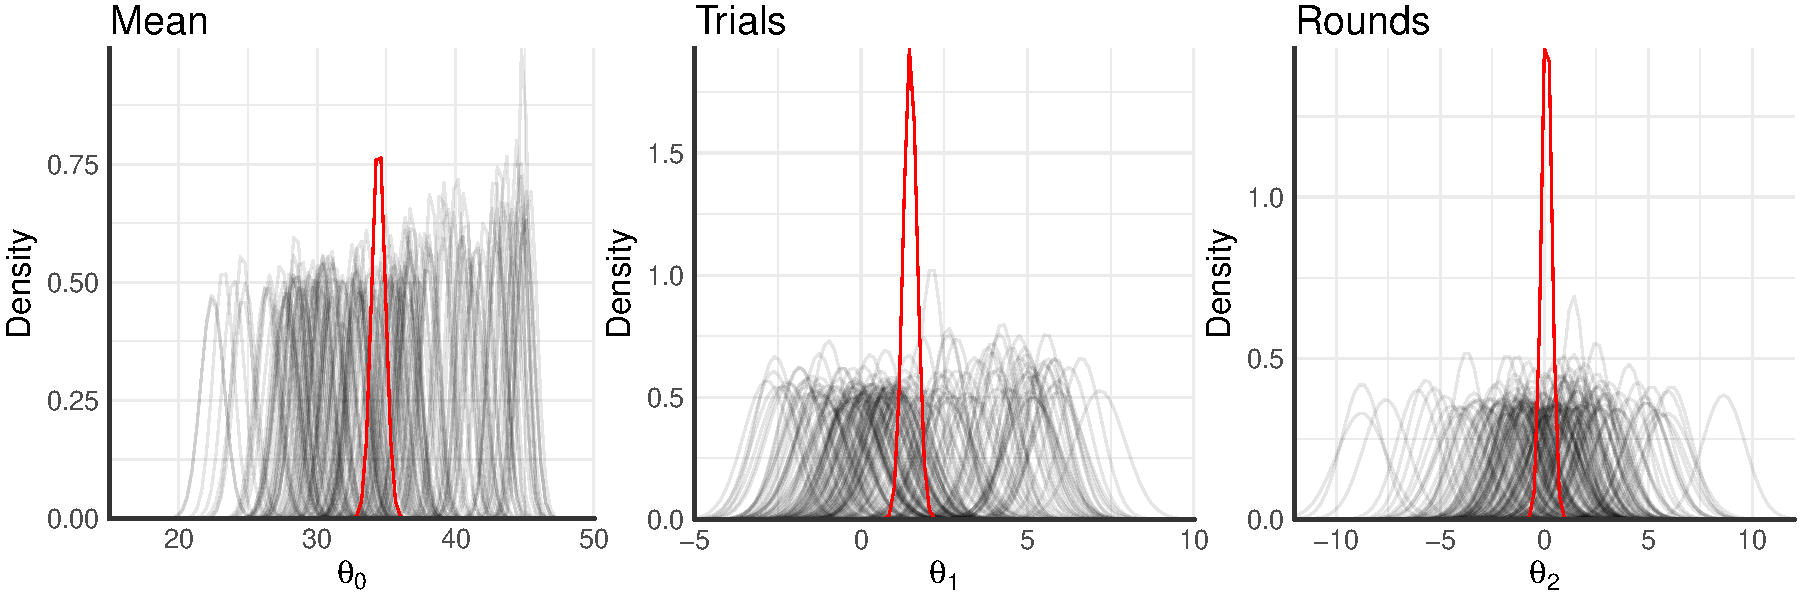
\includegraphics[width=0.8\linewidth]{trialsandrounds.pdf}
\caption{Posterior regression coefficients of mean performance and the effects of both trials and rounds onto participants' rewards. Individual lines densities correspond to participant-wise estimates, whereas red lines show hierarchical estimates.} 
\label{fig:trialandrounds}
\vspace{-1mm}
\end{figure}
We analyze participants learning over trials and rounds using a hierarchical Bayesian regression approach. Formally, we assume the regression weight parameters $\theta_x$ for $x\in\{0,1,2\}$ are hierarchically distributed as
\begin{equation}
\theta_{x} \sim \mathcal{N}(\mu_x, \sigma_{x}^2); 
\end{equation}
we further assume a weakly informative prior of the means and standard deviation over the regression equation, defined as:
\begin{equation}
\mu_x \sim \mathcal{N}(0, 100) 
\label{eqn:hier_mean}
\end{equation}
\begin{equation}
\sigma_{x}^2 \sim \text{Half-Cauchy}(0, 100) 
\end{equation}

We fit one hierarchical model of means and standard deviations over all participants using Hamiltonian Markov chain Monte Carlo sampling as implemented in the \texttt{PyMC}-environment. This yields hierarchical estimates for each regression coefficient overall as well as individual estimates for each participant. Doing so for a model containing an intercept (mean performance), a standardized coefficient of the effect of trials on rewards, as well as a standardized coefficient of the effect of rounds on rewards results into the posterior distributions shown in Figure~\ref{fig:trialandrounds}. 

The overall posterior mean of participants' rewards is estimated to be $34.4$ with a 95\%-credible set of $[33.5,35.4]$. The standardized effect of trials onto rewards is estimated to be $1.48$ with a 95\%-credible set of $[1.1,1.9]$, indicating a strong effect of learning over trials. The standardized effect of rounds onto participants' rewards is estimated to be $0.11$ with a 95\% credible set of $[-0.4,0.6]$, indicating no effect. Taken together, these results indicate that participants performed well above the chance-level of $25$ overall and improved their score greatly over trials. They did not, however, learn or adapt their strategies across rounds. 




\subsection*{Reaction times}
\begin{figure}[ht!]
\centering
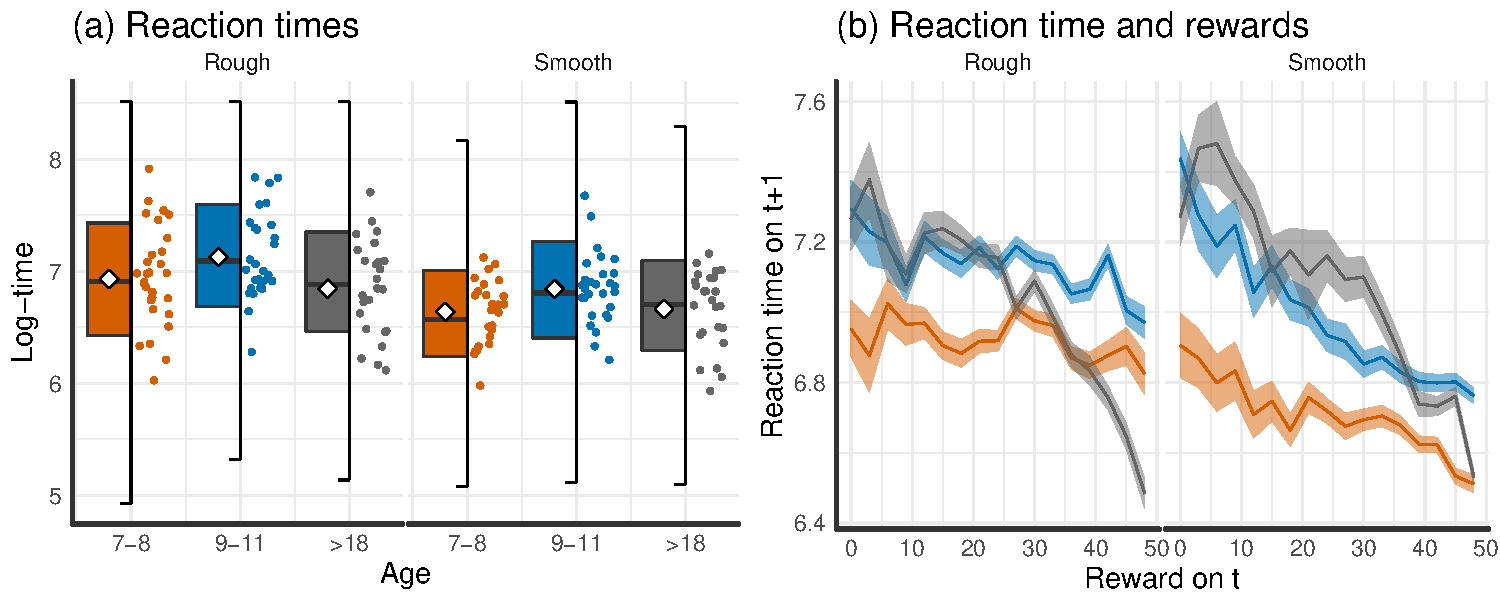
\includegraphics[width=0.8\linewidth]{reactiontimes.pdf}
\caption{Log-reaction times. (a) Reaction time by age group and condition. (b) Reaction times as a function of previous reward.} 
\label{fig:rts}
\vspace{-1mm}
\end{figure}
We analyze participants log-reaction times as function of previous reward, age group, and condition. Reaction times are filtered to be smaller than 5000ms and larger than 100ms (3.05\% removed in total). We find that reaction times are larger for the rough as compared to the smooth condition (see Fig.~\ref{fig:rts}a; $t(158)=4.44$, $p<.001$, $d= 0.70$, 95\% CI=$[0.38, 1.02]$, $BF>10$). Moreover, adults are somewhat faster than children of age 9-11 ($t(103)=-2.60$, 95\% CI=$[0.12, 0.90]$, $p=.01$, $d=0.51$, $BF=4$). The difference in reaction times between children of age 9-11 and children of age 7-8 is only small ($t(108)=2.27,$ $p=.03$, $d=0.43$, 95\% CI=$[0.05, 0.81]$, $BF= 1.97$). 

We also analyze how much a previously found reward influences participants' reaction times, i.e. whether participants slow down after a bad outcome and/or speed up after a good outcome (see Fig.~\ref{fig:rts}b). The correlation between the previous reward and reaction times is negative overall with $r=-0.18$, 95\% CI=$[-0.23, -0.13]$, $t(159)=-15$, $p<.001$, $BF>100$, indicating that larger rewards lead to faster reaction times, whereas participants might slow down after having experienced low rewards. This effect is even stronger for the smooth as compared to the rough condition ($t(158)=-4.43$, $p<.001$, $d=0.70$, 95\% CI=$[0.38, 1.02]$, $BF>100$). Moreover, this effect is also stronger for adults than for older children ($t(103)=-5.51$, $p<.001$, $d=1.08$, 95\% CI=$[0.67, 1.49]$, $BF>100$) and does not differ between the two groups of children ($t(108)=1.93$, $p=.06$, $d=0.37$, 95\% CI=$[-0.01, 0.75]$, $BF=1.05$). 

\begin{figure}[ht!]
\centering
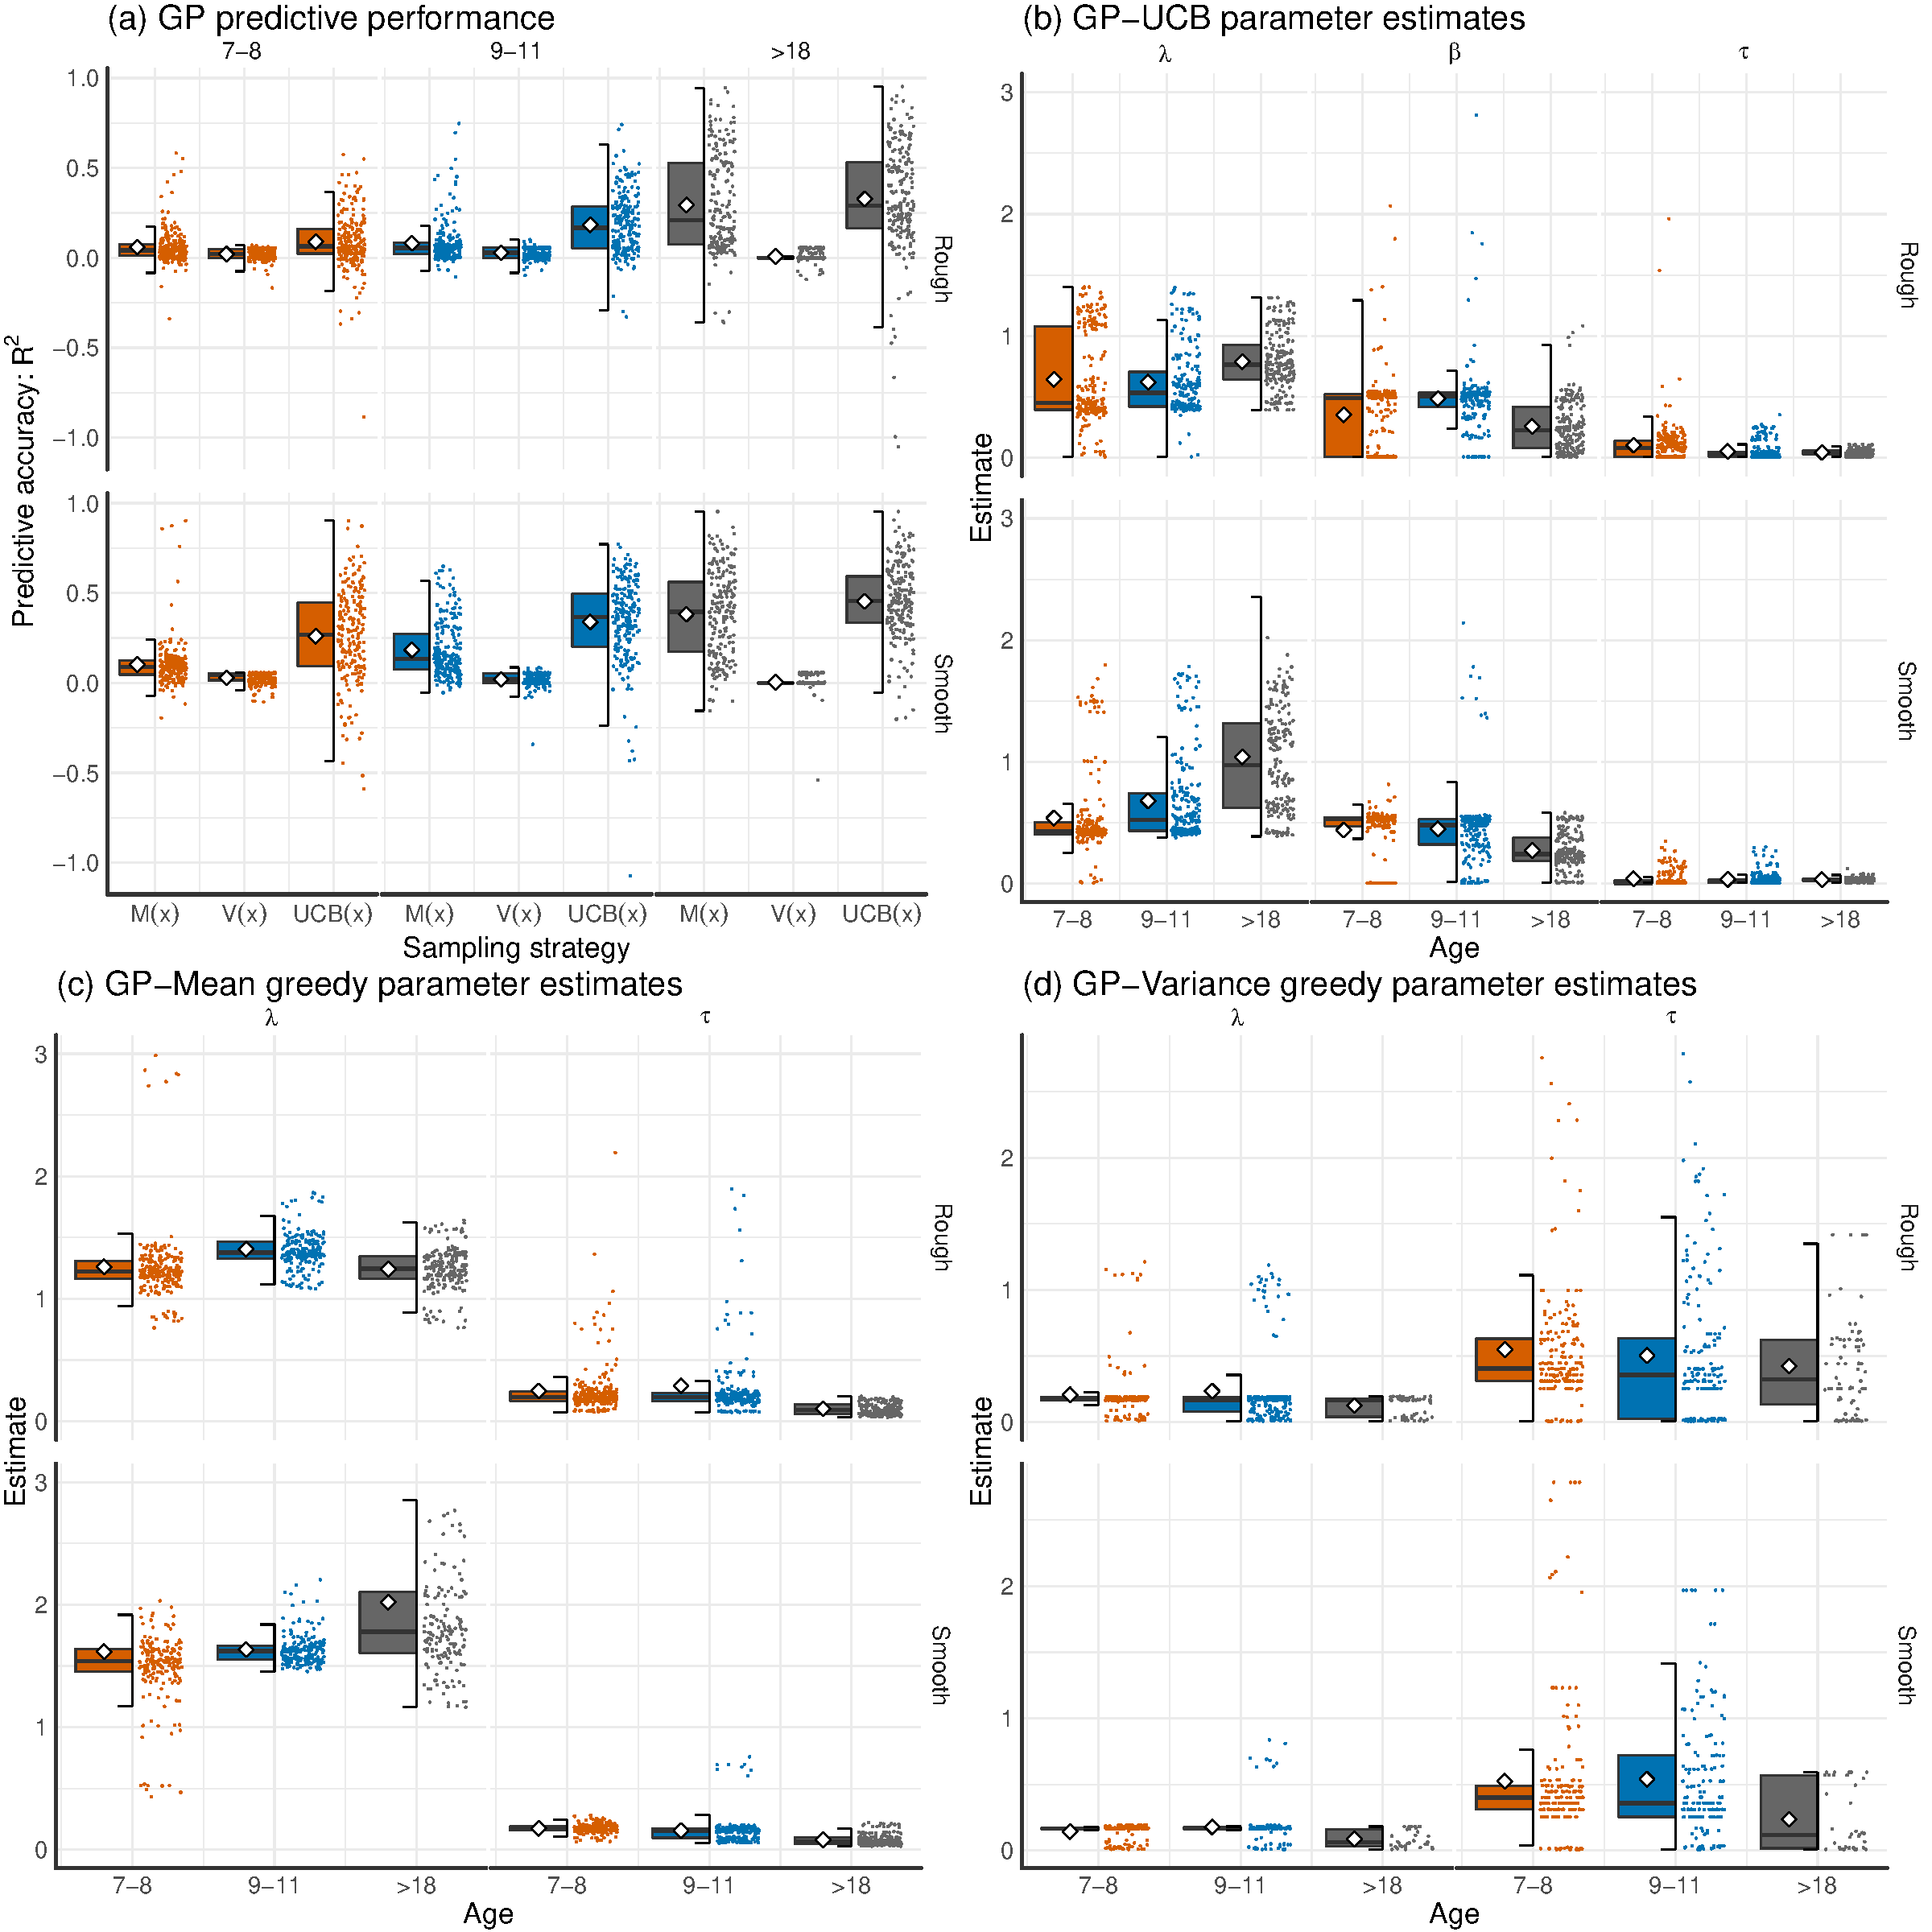
\includegraphics[width=0.9\linewidth]{fullgp.pdf}
\caption{Predictive accuracy ($R^2$) and parameter estimates for the different Gaussian Process-models by age group and condition. All Tukey box plots include raw data points and mean shown as diamond.} 
\label{fig:gpfull}
\vspace{-1mm}
\end{figure}

\begin{figure}[ht!]
\centering
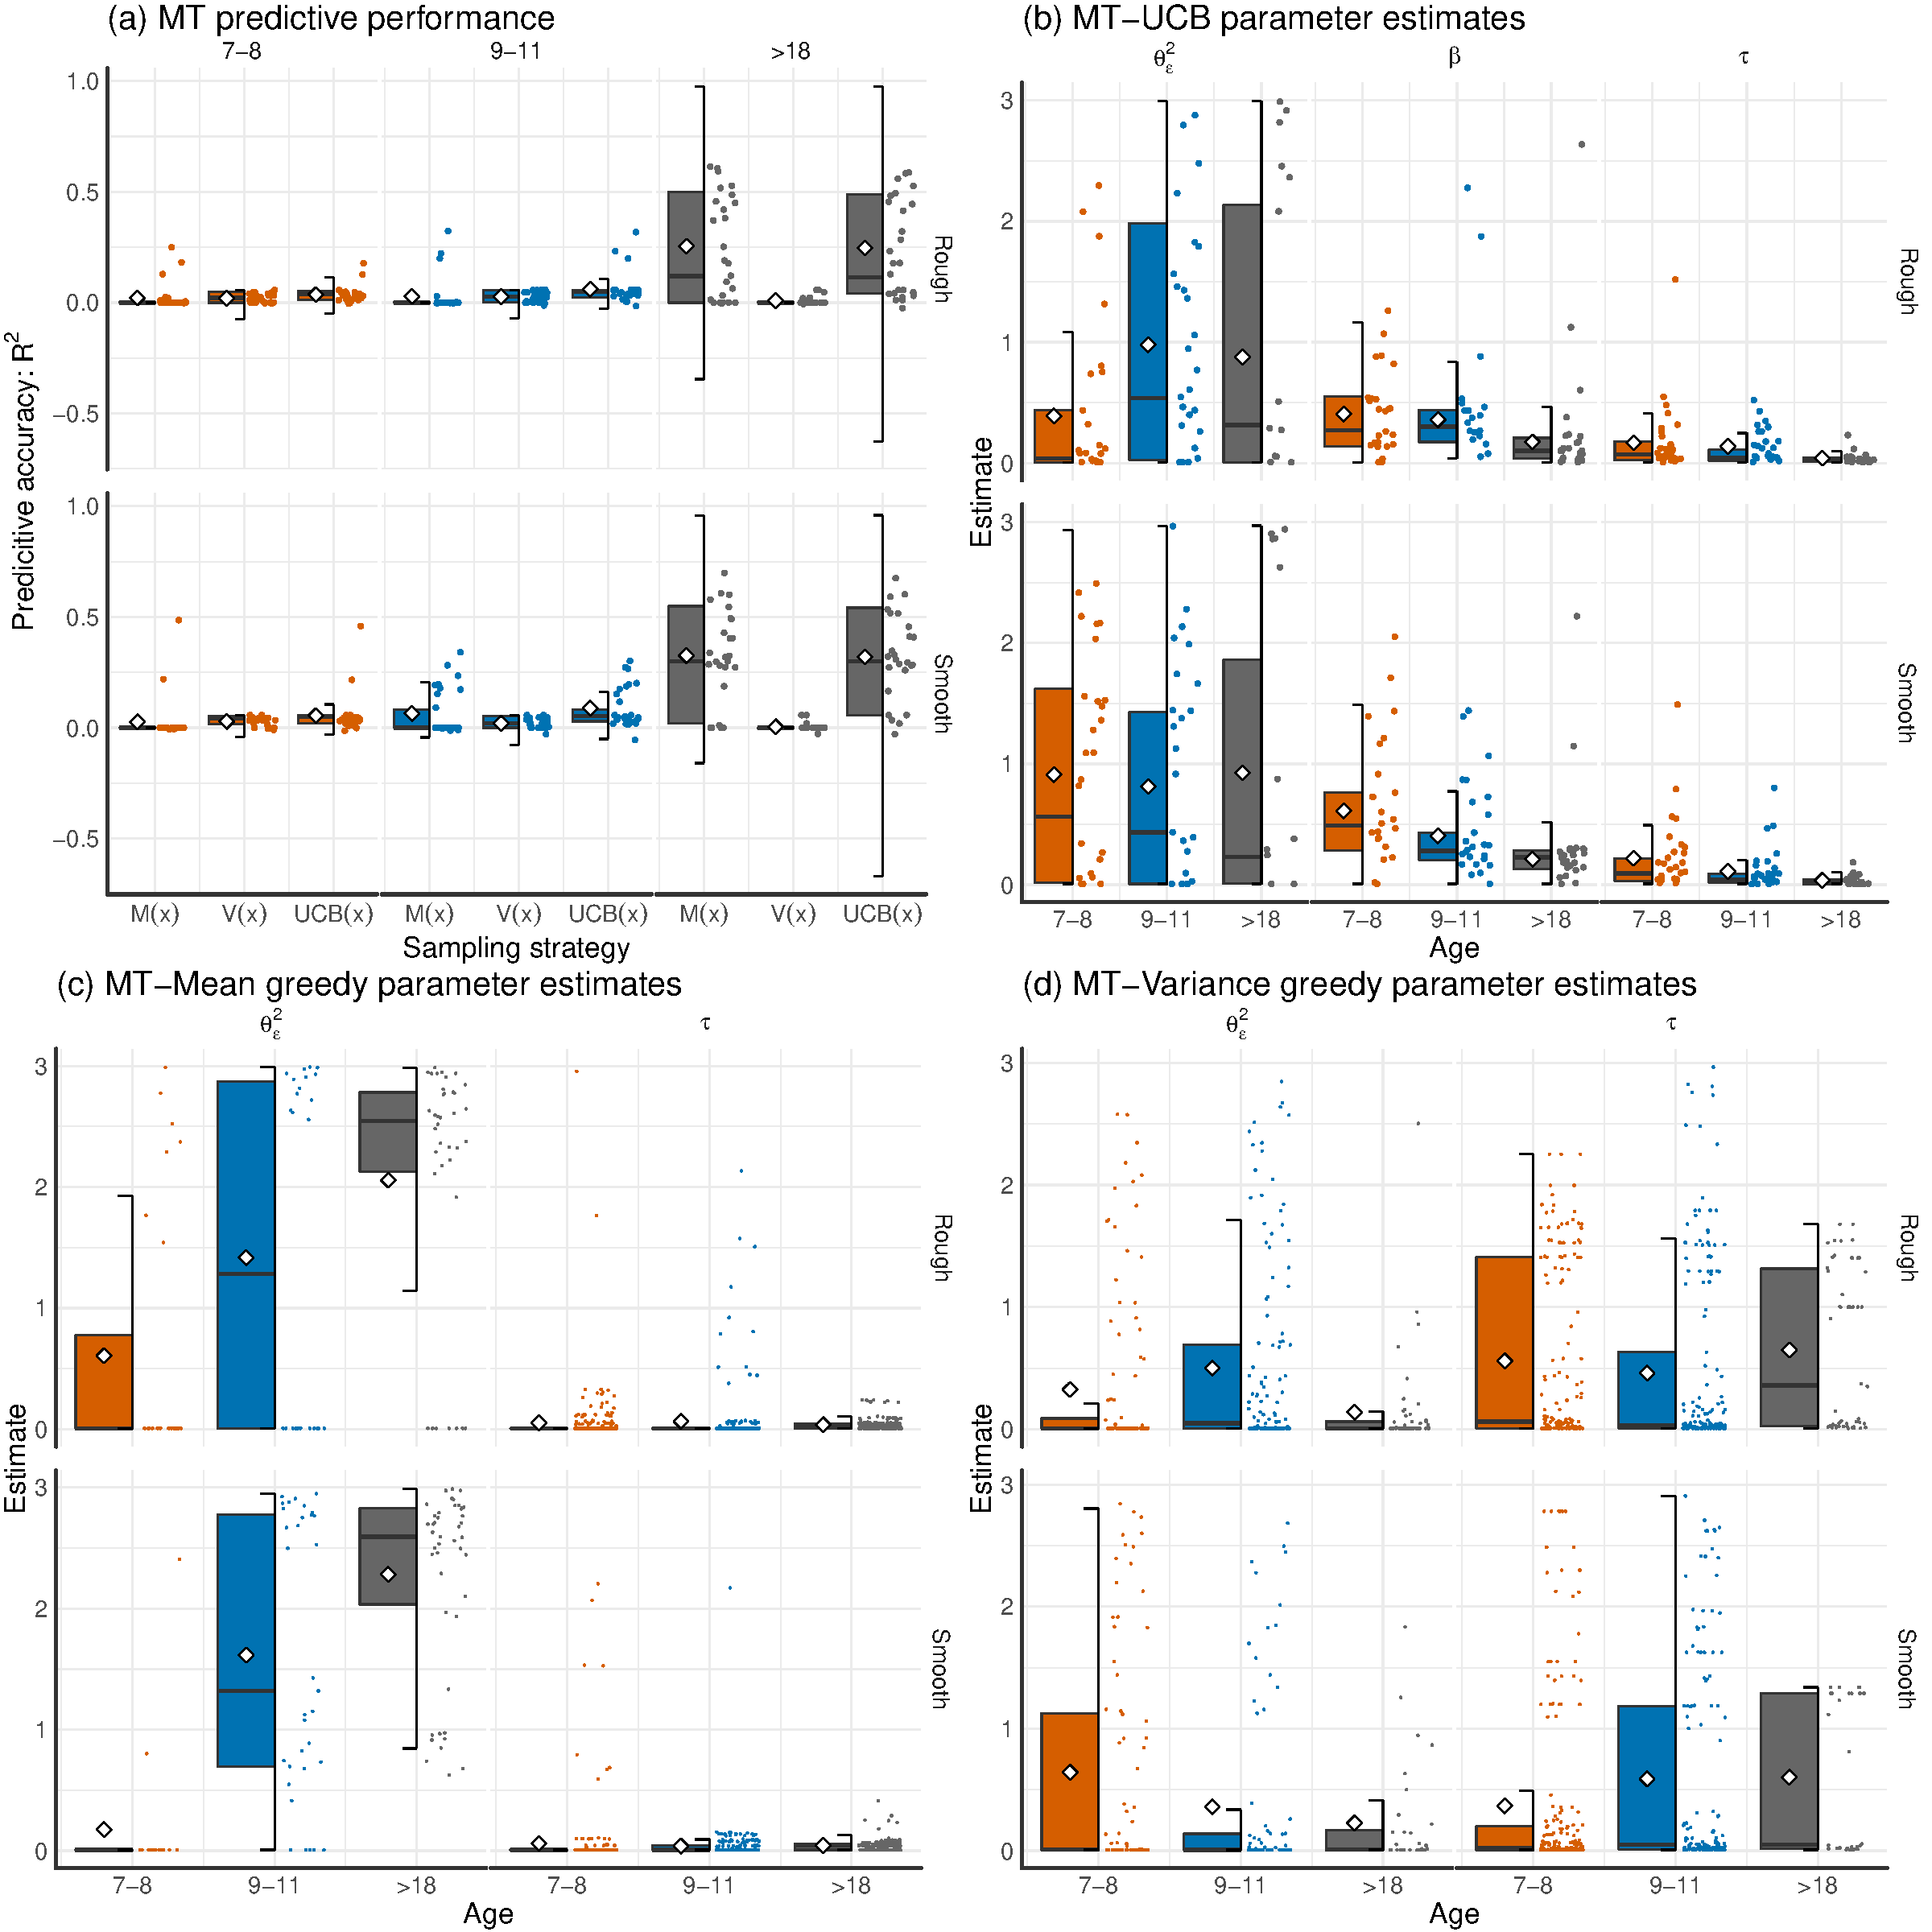
\includegraphics[width=0.9\linewidth]{fullmt.pdf}
\caption{Predictive accuracy ($R^2$) and parameter estimates for the different Bayesian Mean Tracker-models by age group and condition. All Tukey box plots include raw data points and mean shown as diamond.} 
\label{fig:mtfull}
\vspace{-1mm}
\end{figure}


\begin{table*}[ht!]
\centering
 \hfill
 \footnotesize
%\setlength{\tabcolsep}{2.5pt}
\caption{Full modeling results.}
\label{tab:modelResults}
\renewcommand{\arraystretch}{0.9}
\resizebox{\columnwidth}{!}{%
\begin{tabular}{llrrrrrrrrrrrr}
\toprule
\multirow{ 2}{*}{ } & \multirow{ 2}{*}{Model}  &\multirow{ 2}{*}{ }  & \multirow{ 2}{*}{$R^2$}  & \multirowcell{2}{\# Best}  & \multirow{ 2}{*}{Log-loss} & \multirowcell{ 2}{Pr. of \\Exceed.} &\multirow{ 2}{*}{ }  & \multirowcell{ 2}{Generalization\\ $\lambda$}   & \multirowcell{ 2}{Exploration \\$\beta$}  & \multirowcell{ 2}{Error Var.\\ $\sqrt{\theta_\epsilon^2}$}  & \multirowcell{ 2}{Softmax\\$\tau$ }   \\ \\
\midrule
\multicolumn{2}{l}{\textbf{Overall:}}&&&&&&    &  &  &      &      &      &     \\
 & MT-Mean greedy     & & 0.02 & 10  & 103.9  & 0 &   &  --   & --    & 2.98 & 0.01\\
 & MT-Variance greedy & & 0.01 & 3   & 102.7 & 0 &   &  --   & --    & 0.58 & 0.08\\
 & MT-UCB             & & 0.05 & 5   & 99.3  & 0 &   &  --   & 0.41 & 1.60 & 0.16\\
 & GP-Mean greedy     & & 0.09 & 34  & 94.4  & 0 &   & 1.46 & --    & --    & 0.16\\
 & GP-Variance greedy & & 0.02 & 2   & 102.1 & 0 &   & 0.18 & --    & --    & 0.56\\
 & GP-UCB             & & 0.28 & 106 & 74.8  & 1 &   & 0.59 & 0.45 & --    & 0.03\\
\multicolumn{2}{l}{\textbf{Age 7-8:}} &&&&&&&   &   &      &      &      &     \\
 & MT-Mean greedy     && 0.00 & 3  & 103.9  & 0 &  &  --   & --    & 0.53 & 0.01\\
 & MT-Variance greedy && 0.00 & 3  & 100.8 & 0 &  &  --   & --    & 1.22 & 0.08\\
 & MT-UCB             && 0.03 & 3  & 100.5 & 0 &  &  --   & 0.47 & 1.20 & 0.11\\
 & GP-Mean greedy     && 0.07 & 14 & 96.9  & 0 &  & 1.37 & --    & --    & 0.18\\
 & GP-Variance greedy && 0.01 & 0  & 102.7 & 0 &  & 0.17 & --    & --    & 0.41\\
 & GP-UCB             && 0.14 & 32 & 89.2  & 1 &  & 0.46 & 0.48 & --    & 0.03\\
\multicolumn{2}{l}{\textbf{Age 9-11:}}&&&&&&&  &  &      &      &      &     \\
 & MT-Mean greedy     && 0.01 & 0  & 103.9  & 0 &  &  --   & --    & 2.86 & 0.01\\
 & MT-Variance greedy && 0.01 & 0  & 101.7 & 0 &  &  --   & --    & 0.65 & 0.08\\
 & MT-UCB             && 0.05 & 0  & 99.3  & 0 &  &  --   & 0.33 & 1.34 & 0.07\\
 & GP-Mean greedy     && 0.08 & 9  & 95.1  & 0 &  & 1.52 & --    & --    & 0.17\\
 & GP-Variance greedy && 0.01 & 2  & 101.5 & 0 &  & 0.17 & --    & --    & 0.38\\
 & GP-UCB             && 0.26 & 44 & 76.6  & 1 &  & 0.74 & 0.53 & --    & 0.02\\
\multicolumn{2}{l}{\textbf{Adults:}} &&  &  &  &  &  &  &  &  &  &  & \\
 & MT-Mean greedy     && 0.29 & 7  & 72.8  & 0 &  &  --   & --    & 3.38 & 0.03\\
 & MT-Variance greedy && 0.00 & 0  & 103.4 & 0 &  &  --   & --    & 0.13 & 0.87\\
 & MT-UCB             && 0.29 & 2  & 74.2  & 0 &  &  --   & 0.18 & 2.94 & 0.03\\
 & GP-Mean greedy     && 0.33 & 11 & 69.1  & 0 &  & 1.38 & --    & --    & 0.07\\
 & GP-Variance greedy && 0.01 & 0  & 103.9 & 0 &  & 0.10 & --    & --    & 0.23\\
 & GP-UCB             && 0.40 & 30 & 62.7  & 1 &   & 0.85 & 0.24 & --    & 0.03\\
 \midrule
 \multicolumn{14}{p{18cm}}{\textit{Note}: Columns indicate (from left to right) the average predictive accuracy of each model ($R^2$), how many participants each model best predicted  (\# Best), the average log-loss over all 8 rounds of predictions (Log-loss), the protected probability of exceedance (Pr. of Exceed.), the GP's generalization parameter ($\lambda$), the directed exploration parameter ($\beta$) for all models involving a UCB sampling strategy, the MT's error variance ($\sqrt{\theta_\epsilon^2}$), and the random exploration (softmax temperature) parameter ($\tau$). Parameter estimates are based on median over per-participant mean parameter estimates (excluding estimates larger than 5 as outliers).}\\
\bottomrule
\end{tabular}}
\end{table*}
